\cotefile{148}
\scanpage{11}
\mspage{4}

The group $\mathbb Z/6\mathbb Z$ acts \unsure{transitive\textsuperscript{ly}|transitively} on $({}_2X_S)\setminus\{0\}$ for $\pm1$ acts trivially - thus ${}_2X_S\setminus\{0\}$ is a torsor under
\[
(\mathbb Z/6\mathbb Z)/\pm1\simeq\mathbb Z/3\mathbb Z
\]
\deleted{\unsure{(conj.|conj.}} (corresponding generator $\unsure{\simeq|=}\,-\bar\zeta\,\unsure{j|\zeta}=\exp\frac{2\pi}{6}$),
\deleted{\unsure{in this case|in cor|in cov} \unsure{torsor|C by}} \inserted{\unsure{the|this|a} torsor} is identified : $S/\pm1$, by
% Source-state: two short crossed strokes beneath a raised replacement a;
% the old strokes are reproduced without assigning them a letter value.
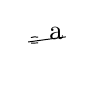
\begin{tikzpicture}[baseline={(0,0)},x=1em,y=1ex,line width=.35pt]
  \draw (.08,2.25) .. controls (.16,2.33) and (.25,2.32) .. (.34,2.28);
  \draw (.09,1.78) -- (.34,1.80);
  \draw (-.02,1.88) -- (1.34,2.31);
  \node[anchor=base,inner sep=0pt] at (.99,2.08) {\inserted{a}};
\end{tikzpicture}ssociating \unsure{:|to} each $s\in S$ the midpoint of the radius $[0,s]$, or rather its image in\inserted{)} $X_S$.

The set of fixed points of $\mathbb Z/3\mathbb Z\inserted{\subset\mathbb Z/6\mathbb Z}$ on $X_S$ is of cardinality 3, it is obtained by taking the \unsure{barycentres} of the six triangles of the central (bibarycentric) subdivision of the hexagon (circled points) (\unsure{such as|such as} $(1-\bar\zeta)/3$ and so on in the pinned case), they group into two packets of 3 \unsure{mutual\textsuperscript{ly}|mutually} congruent under $\Gamma$, \unsure{giving|give} two elements (symmetric) of $X_S$, of order 3,

\margin{10}
